\documentclass[a4paper]{sciposter}
\usepackage{lipsum}
\usepackage{epsfig}
\usepackage{amsmath}
\usepackage{amssymb}
\usepackage{amsthm}
\usepackage[catalan]{babel}
\usepackage{geometry}
\usepackage{multirow}
\usepackage{multicol}
\usepackage{graphicx}
\usepackage{tikz}
\usepackage{wrapfig}
\usepackage{gensymb}
\usepackage[utf8]{inputenc}
\usepackage{empheq}
\usepackage{letltxmacro}

\graphicspath{{images/}}

\newtheorem{teorema}{Teorema}

\makeatletter
\def\timeframe#1{\def\@timeframe{#1}}
\def\period#1{\def\@period{#1}}
\let\oldr@@t\r@@t
\def\r@@t#1#2{
\setbox0=\hbox{$\oldr@@t#1{#2\,}$}\dimen0=\ht0
\advance\dimen0-0.2\ht0
\setbox2=\hbox{\vrule height\ht0 depth -\dimen0}
{\box0\lower0.4pt\box2}}
\LetLtxMacro{\oldsqrt}{\sqrt}
\renewcommand*{\sqrt}[2][\ ]{\oldsqrt[#1]{#2} }
\makeatother

\geometry{
 landscape,
 a1paper,
 left=5mm,
 right=50mm,
 top=5mm,
 bottom=50mm,
}
\newcommand*\widefbox[1]{\fbox{\hspace{2em}#1\hspace{2em}}}

\newlength\dlf  % Define a new measure, dlf
\newcommand\alignedbox[2]{
% Argument #1 = before & if there were no box (lhs)
% Argument #2 = after & if there were no box (rhs)
&  % Alignment sign of the line
{
\settowidth\dlf{$\displaystyle #1$}
    % The width of \dlf is the width of the lhs, with a displaystyle font
\addtolength\dlf{\fboxsep+\fboxrule}
    % Add to it the distance to the box, and the width of the line of the box
\hspace{-\dlf}
    % Move everything dlf units to the left, so that & #1 #2 is aligned under #1 & #2
\boxed{#1 #2}
    % Put a box around lhs and rhs
}
}

\usepackage{titlesec}
\titleformat{\section}[block]{\LARGE\bfseries\centering}{}{1em}{\color{blue}}
\titleformat{\subsection}[block]{\Large\bfseries\centering}{}{1em}{\color{blue}}
\titleformat{\subsubsection}[block]{\large\bfseries\centering}{}{1em}{\color{blue}}

\usepackage{graphicx,url}

\begin{document}
\fontfamily{phv}\selectfont

\begin{multicols}{3}
\section{Introducció}
Recordatori de conceptes bàsics de probabilitat i estadística.\\
Una \textbf{població} es una variable aleatoria $X$.\\
Una \textbf{mostra aleatòria} de mida $n$ de $X$ és un conjunt de variables aleatòries $X_1,\dots,X_n$ independents i que compleixen el seguent $\forall A\subset\mathbb{R}, i \in 1,\dots,n:P(X_i \in A) = P(X\in A)$\\
Els \textbf{paràmetres} són característiques numèriques poblacionals que solen ser desconegudes, com
\begin{itemize}
	\item La mitjana $\mu = E(X)$
	\item La variància $\sigma^2 = Var(X)$
	\item La desviació estàndard $\sigma = \sqrt{Var(X)}$
\end{itemize}
\subsection{Estadistics}
Donada una mostra aleatòria $X_1,\dots,X_n$ de $X$, un \textbf{estadístic} és una funció d'aquestes variables, i potser de constants conegudes.\\
\textbf{Exemples:}
La mitjana mostral $\overline{x} = \frac{1}{n} \sum\limits_{i=1}^{n} x_i$.\\
La variància mostral (corregida) $S^2 = \frac{1}{n-1} \sum\limits_{i=1}^{n} (x_i - \overline{x})^2$.\\
La variància mostral (no corregida) $S'^2 = \frac{n-1}{n}S^2$.\\
La quasi-variància mostral $\tilde{S}^2 = \frac{1}{n} \sum\limits_{i=1}^{n} (x_i - \mu)^2$ on $\mu$ és la mitjana poblacional de $X$.
\subsection{Estimadors}
Un \textbf{estimador} és un estadístic que es fa servir per estimar un determinat parametre.\\
Notació: Un estadístic que s'usa per estimar el paràmetre $\theta$ es denotat com $\hat{\theta}$. Llavors tenim
\begin{itemize}
	\item $\hat{\mu} = \overline{X}$.
	\item $\hat{\sigma}^2 = S^2$.
\end{itemize}
Distingim entre \textbf{estimadors} (és variable aleatòria) i \textbf{estimació} (valor concret, que es la seva realització, en minúscula).
\subsection{Distrubucions mostrals més usuals}
Donat un estadístic funció de la mostra $X_1,\dots,X_n$ que és una variable aleatòria, la seva distribució és la \textbf{distribució de mostral de l'estadístic}.\\
Propietats de la llei de la mitjana mostral:
\begin{itemize}
	\item $\mu_{\overline{X}} = E(\overline{X}) = \mu$.
	\item $\sigma^2_{\overline{X}} = Var(\overline{X}) = \frac{\sigma^2}{n}$.
\end{itemize}
Si $X \sim N(\mu,\sigma^2)$, aleshores $\overline{X} \sim N(\mu,\frac{\sigma^2}{n})$.\\
Propietats de la llei de la variància mostral (corregida), sense corregir i quasivariància:
\begin{itemize}
	\item $E(\tilde{S}^2) = \sigma^2$.
	\item $E(S^2) = \sigma^2$.
	\item $E(S'^2) = \frac{n-1}{n}\sigma^2$.
\end{itemize}
Si $X \sim N(\mu,\sigma^2)$, aleshores $\frac{n\tilde{S}^2}{\sigma^2} = \frac{1}{\sigma^2} \sim^n_{i=1}(X_1-\mu)^2 \sim \chi^2_n$, on $\chi^2_n$ és la distribució khi-quadrat amb $n$ graus de llibertat. Això es fa servir si $\mu$ és coneguda.\\
\begin{teorema}[Teorema de Fisher]
Si $X_1, \dots, X_n$ és una mostra aleatòria de $X \sim N(\mu,\sigma^2)$, aleshores:
\begin{enumerate}
	\item $\overline{X}$ i $S^2$ són independents.
	\item A més $\frac{(n-1)S^2}{\sigma^2} = \frac{1}{\sigma^2} \sum\limits_{i=1}^{n} (X_i - \overline{X})^2 \sim \chi^2_{n-1}$.
\end{enumerate}
Aixó es fa servir si $\mu$ és desconeguda.
\end{teorema}
\begin{figure}[H]
    \centering
    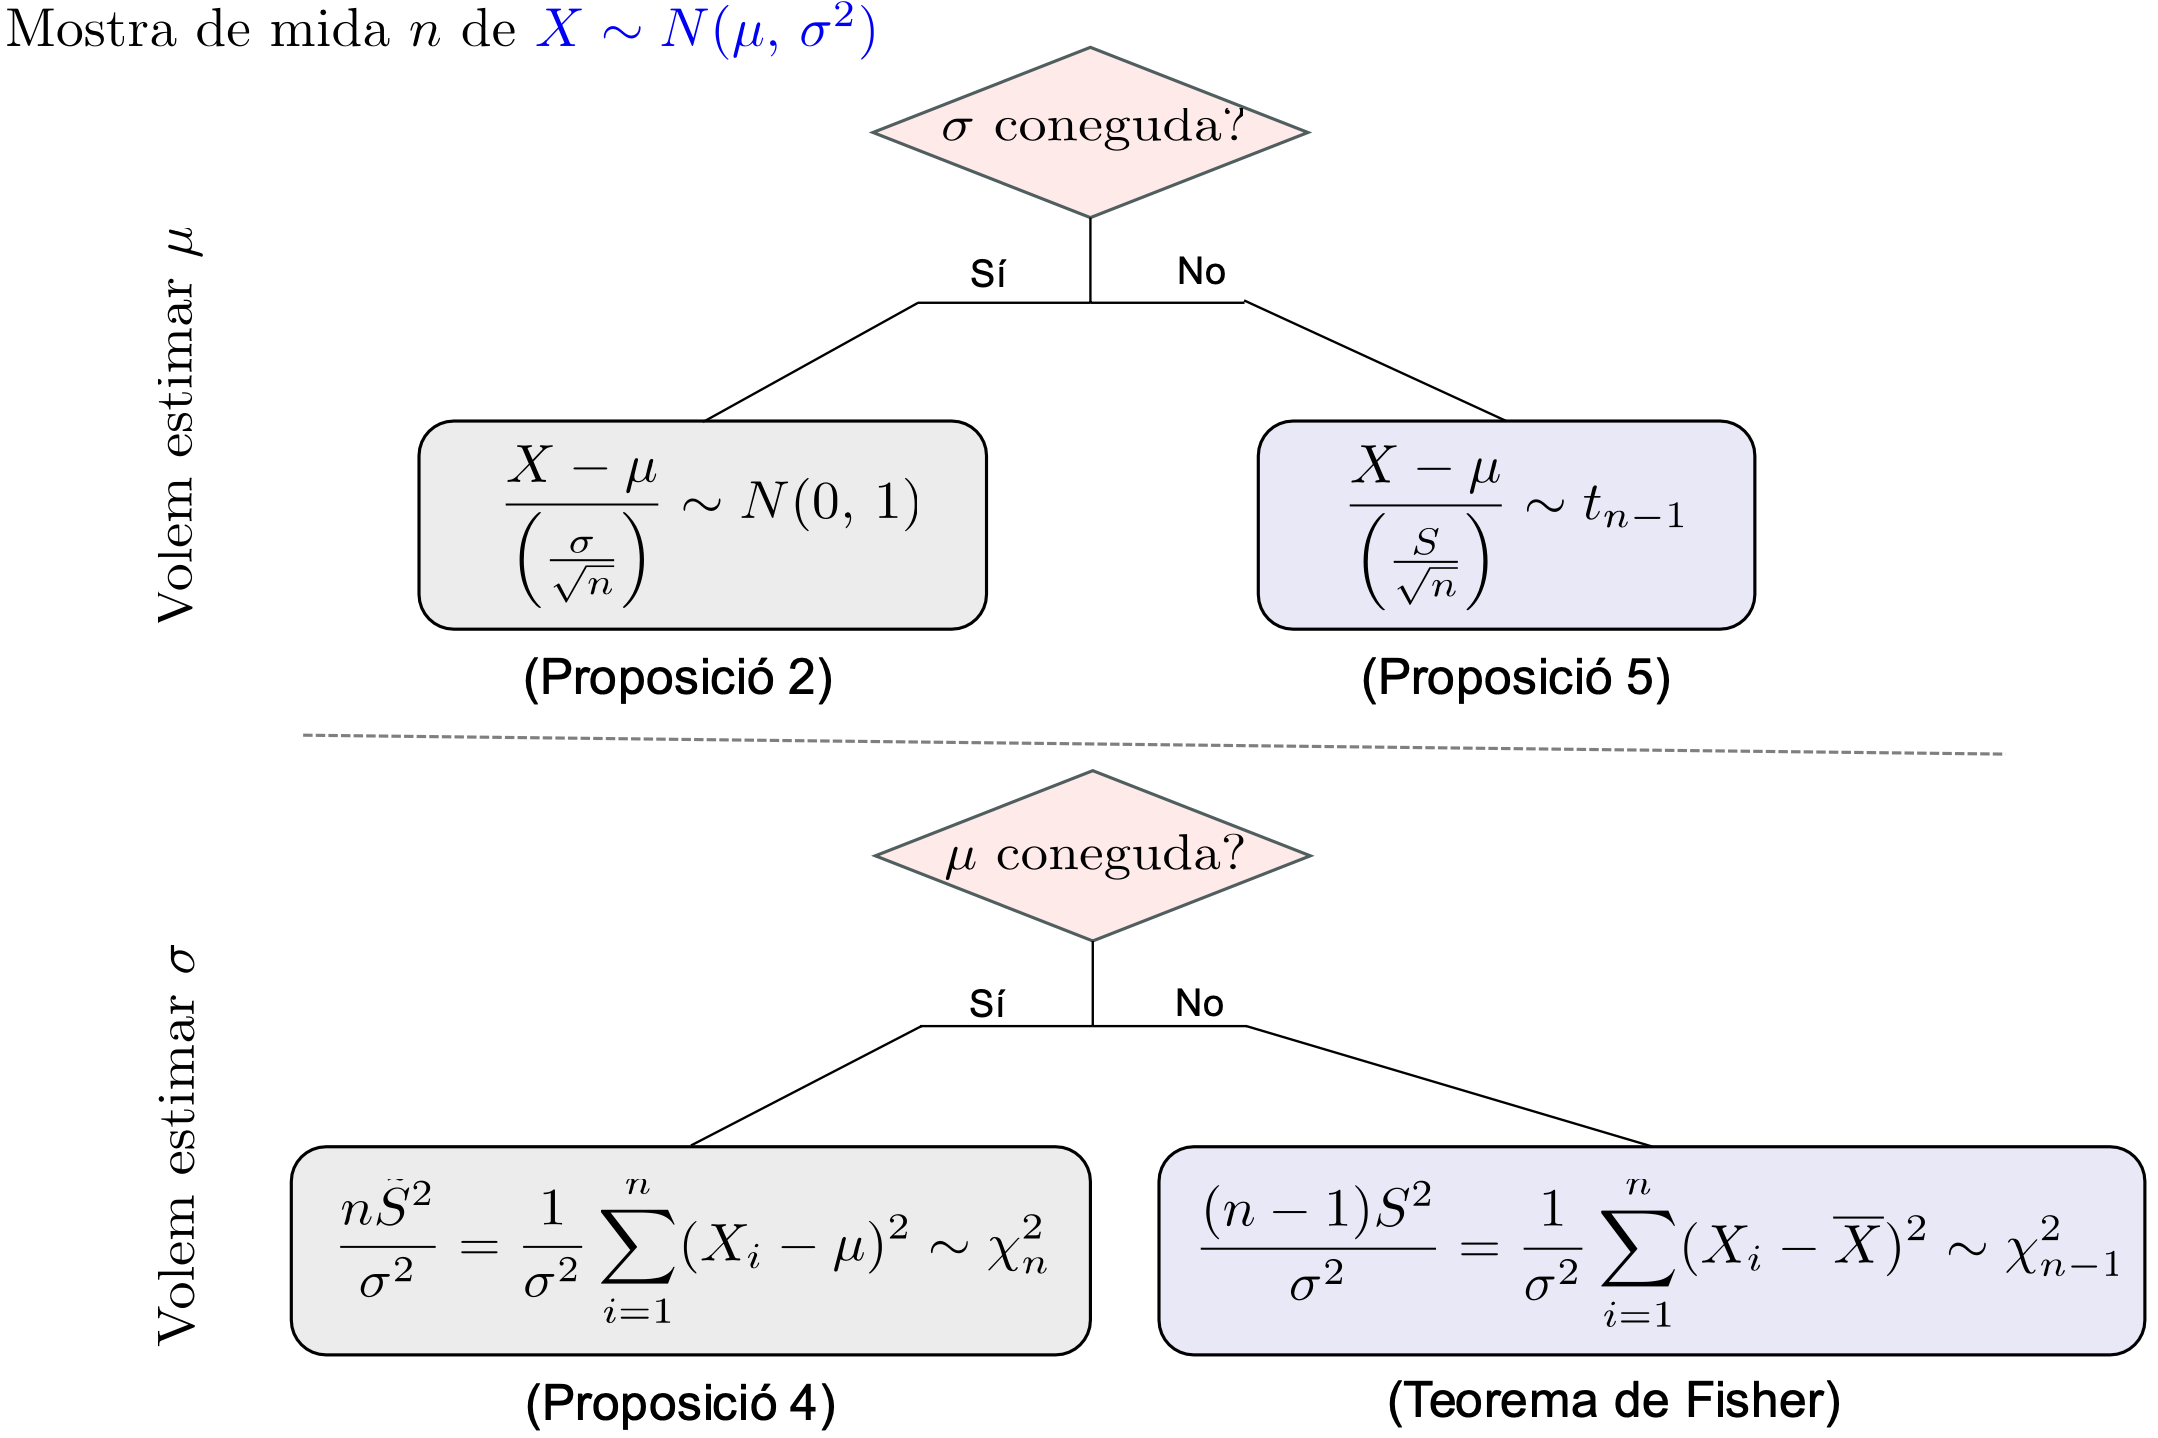
\includegraphics[width=0.8\textwidth]{fix.png}
\end{figure}
Si $X \sim N(\mu, \sigma^2)$ aleshores $T = \frac{\overline{X} - \mu}{\left(\frac{S}{\sqrt{n}}\right)} \sim t_{n-1}$, on $\underbrace{S = +\sqrt{S^2}}_\text{Això es estupid?}$ i $t_{n-1}$ és la distribució t de Student amb $n-1$ graus de llibertat.
\subsection{Distribucions mostrals asimptòtiques}
Si $X_1,\dots,X_n$ és una mostra aleatòria de $X$ amb llei qualsevol i mida $n$ tal que $E(X) = \mu$ i $Var(X) = \sigma^2$, aleshores $\underline{X}_n \approx N\left(\mu, \frac{\sigma^2}{n}\right)$, equivalentment $Z_n = \frac{\overline{X}_n - \mu}{\left(\frac{\sigma}{\sqrt{n}}\right)} \approx N(0,1)$.\\
També si $n$ és prou gran i $\sigma$ és desconeguda, aleshores tenim el seguent $\frac{\overline{X}_n - \mu}{\left(\frac{S_n}{\sqrt{n}}\right)} \approx N(0,1)$. A la majoria de distribucions l'approximació es prou bona a partir de $n \geq 30$.\\
\begin{figure}[H]
	\centering
	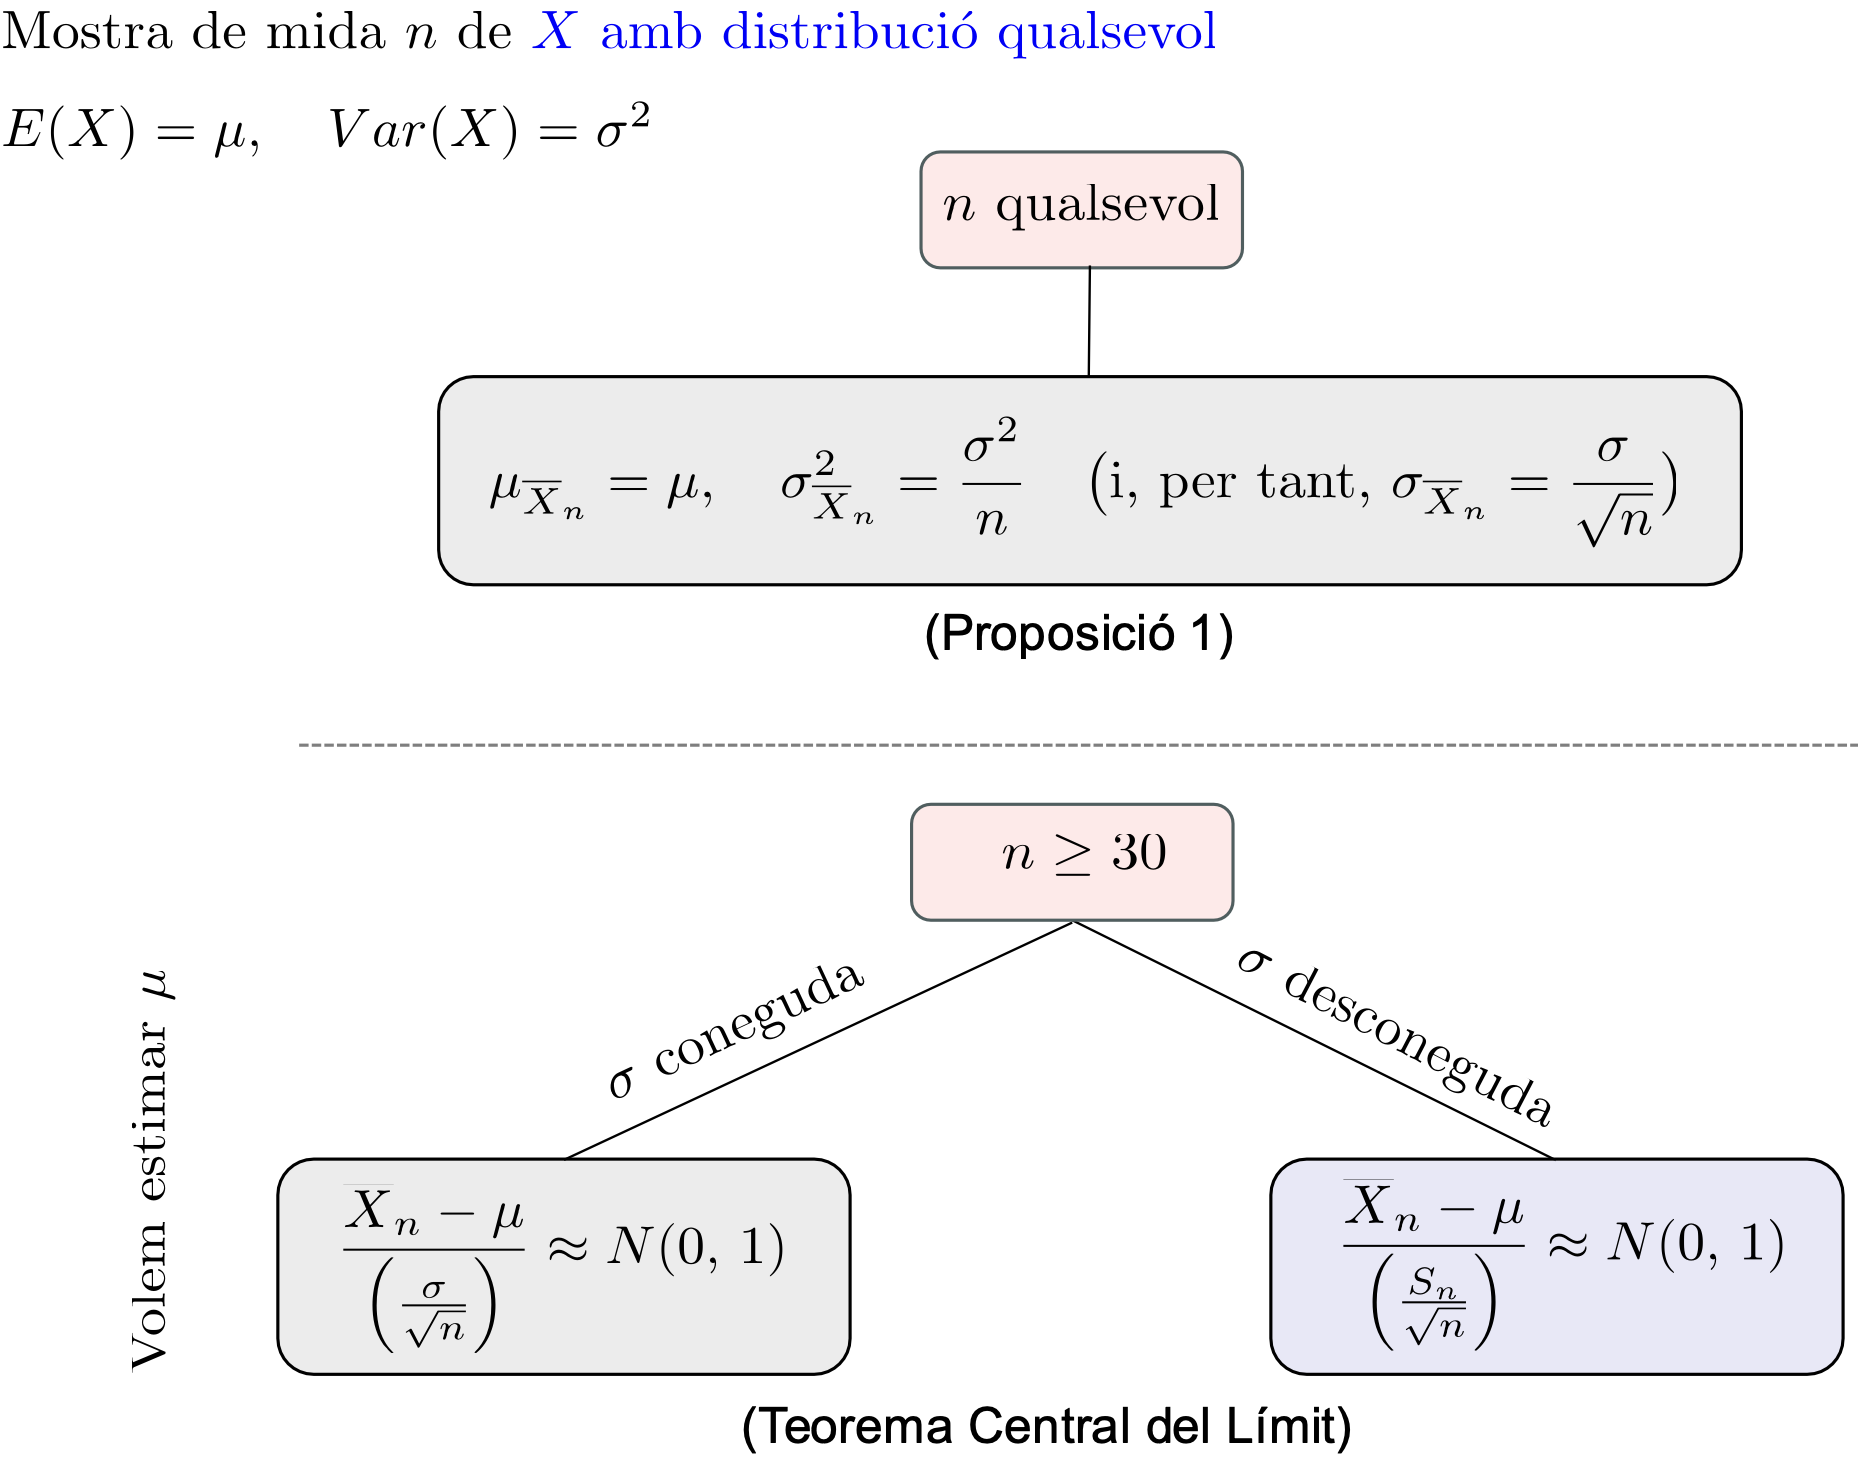
\includegraphics[width=0.8\textwidth]{distro.png}
	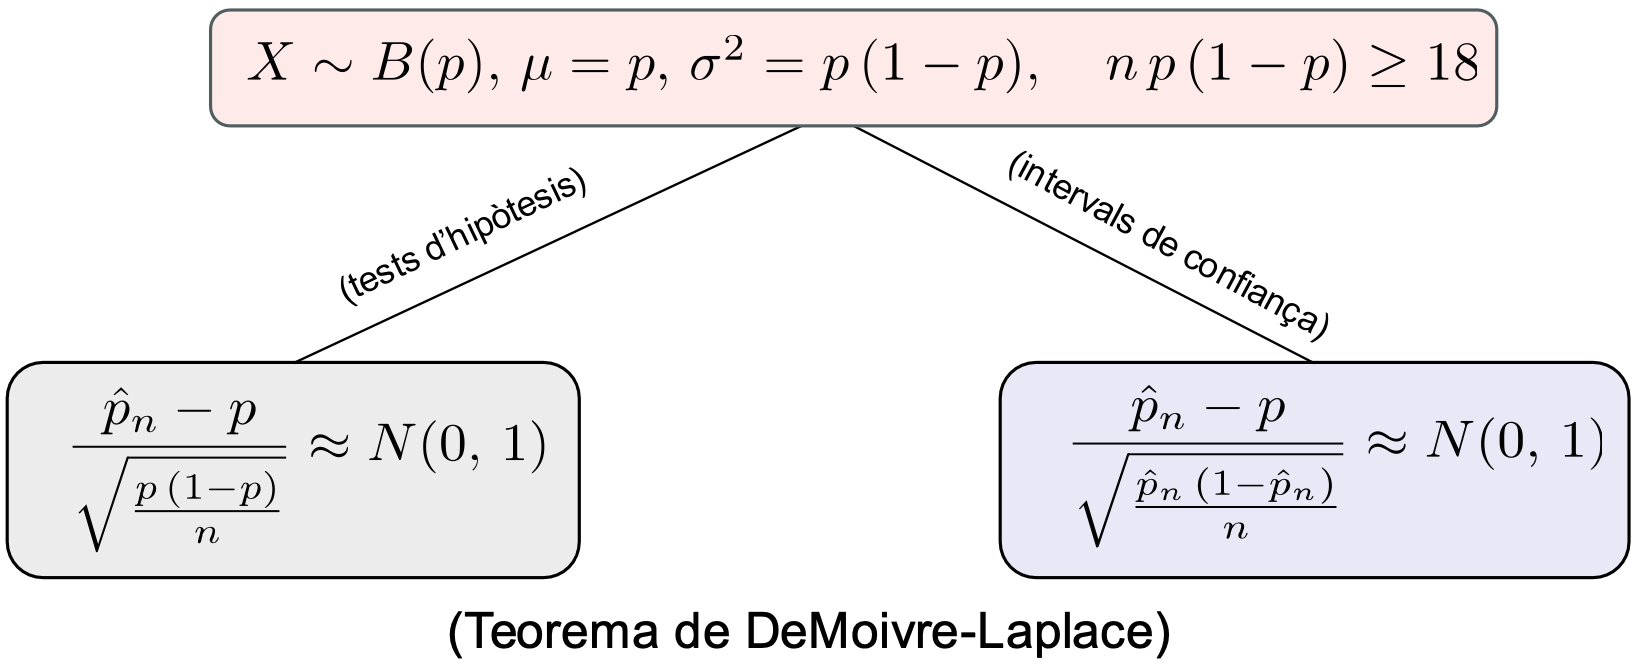
\includegraphics[width=0.8\textwidth]{distro2.png}
\end{figure}
$\frac{\hat{p}_n-p}{\sqrt{\frac{p(1-p)}{n}}} \approx N(0,1)$, on $\hat{p}_n$ és la proporció mostral, $p$ és la proporció poblacional i $n$ és la mida de la mostra.\\
Quan més gran sigui $np(1-p)$ millor es l'aproximació. Es considera acceptable si $np(1-p) \geq 5$.
\subsection{Estadístics d'ordre}
Donada una mostra de mida $n$ de $X$: $X_1,\dots,X_n$, els estadístics d'ordre són les variables aleatòries $X_{(1)},\dots,X_{(n)}$ que són les dades ordenades de menor a major.\\
Exemples importants:
\begin{itemize}
	\item La mediana, el valor que separa la meitat superior de la inferior $Q_2 = \begin{cases}
	X_{((n+1)/2)} & \text{si $n$ és senar} \\
	\frac{X_{(n/2)} + X_{(n/2+1)}}{2} & \text{si $n$ és parell}
	\end{cases}$
	\item Els quartils, els valors que divideixen la mostra en 4 parts iguals: $Q_1 = X_{(n/4)}$, $Q_3 = X_{(3n/4)}$.
	\item El rang interquartílic, $IQR = Q_3 - Q_1$. Ajuda a entendre la dispersió de les dades centrals.
\end{itemize}
Si $X$ és una v.a. amb funció de distribució $F_X$, i $X_1,\dots,X_n$, aleshores la funció de dist. de la v.a. màxim és $F_{X_{(n)}}(t) = (F_X(t))^n\;\forall t \in \mathbb{R}$.\\
Si $X$ és una v.a. amb funció de distribució $F_X$, i $X_1,\dots,X_n$, aleshores la funció de dist. de la v.a. mínim és $F_{X_{(1)}}(t) = 1 - (1 - F_X(t))^n\;\forall t \in \mathbb{R}$.\\
Si $X$ és una v.a. amb funció de distribució $F_X$, i $X_1,\dots,X_n$, aleshores la funció de dist. de la v.a. $k$-èssim és $F_{X_{(k)}}(t) = \sum\limits_{j=k}^{n} \binom{n}{j} (F_X(t))^j (1-F_X(t))^{n-j}\;\forall t \in \mathbb{R}$.
\subsection{Apendix A}
\subsubsection{La distribució $\chi^2$}
Si $Z_1,\dots,Z_n$ són v.a. independents amb distribució $N(0,1)$, aleshores la v.a. $Y = Z_1^2 + \dots + Z_n^2$ llavors $Y \sim \chi^2_n$ amb $n$ graus de llibertat.\\
Propietats:
\begin{itemize}
	\item La variable $Y$ pren valors positius; la seva funció de densitat
	\begin{displaymath}
		f_Y(x) =
		\begin{cases}
			0 & \text{si } x \leq 0 \\
			\frac{1}{2^{n/2}\Gamma(n/2)}x^{n/2-1}e^{-x/2} & \text{si } x > 0
		\end{cases}
	\end{displaymath}
	Amb $\Gamma$ la funció gamma d'Euler.
	\item La seva funció generatriu de moments és $\phi_Y(t) = (1-2t)^{-n/2},\;t<1/2$.
	\item $E(Y) = n$, $Var(Y) = 2n$.
    \item Si $Z \sim N(0,1)$ aleshores $Z^2 \sim \chi^2_1$.
    \item Quan $n$ és suficientment gran es pot fer servir l'aproximació $\sqrt{2\chi^2_n} \approx N(\sqrt{2n-1}, 1)$.
\end{itemize}
\subsubsection{La distribució $t$ de Student}
Si $Z \sim N(0,1)$ i $Y \sim \chi^2_n$ són independents, aleshores la v.a. $T = \frac{Z}{\sqrt{Y/n}}$ $Y \sim t_n$, la $t$ de Student amb $n$ graus de llibertat.\\
Propietats:
\begin{itemize}
	\item La funció de densitat de $T \sim t_n$ és
	\begin{displaymath}
		f_T(x) = \frac{\Gamma\left(\frac{n+1}{2}\right)}{\sqrt{\pi n}\gamma\left(\frac{n}{2}\right)}\left(1+\frac{x^2}{n}\right)^{-\frac{n+1}{2}}
	\end{displaymath}
	\item La densitat de la $t$ de Student és no nul·la en tot $\mathbb{R}$. També és simètrica respecte l'eix vertical. $n \to \infty \Rightarrow t_n \to N(0,1)$.
	\item Si $T \sim t_n$ aleshores $E(T^k)$ només existeix si $k < n$. A més, $E(T) = 0$ si $n > 1$ i $Var(T) = \frac{n}{n-2}$ si $n>2$.
\end{itemize}
\section{Intervals de confiança}
Sigui $X$ una v.a. i $\theta$ qualsevol paràmetre desconegut de la llei de $X$. Fixem un valor $\gamma \in (0,1)$. Un interval de confiança per $\theta$ és una parella de nombres reals $t_1 < t_2$ tals que $\theta$ està entre $t_1$ i $t_2$ amb una confiança de $\gamma$. $\gamma$ és el nivell de confiança de l'interval.\\
Com? Es tracta de trobar dos estadístics $T_1$ i $T_2$ tal que $P(T_1 < \theta < T_2) \geq \gamma$.\\
El metode més comú per trobar intervals de confiança és el mètode del pivot.
\subsection{Mètode del pivot}
Un pivot és una v.a. $T$ tal que és una funció de la mostra i del parametre $\gamma$ i no depén de cap parametre desconegut $T = T(X_1,\dots,X_n;\theta)$. La llei de $T$ és coneguda i no depén de cap paràmetre desconegut excepte $\theta$.
\subsubsection{Per mitjana normal amb variància coneguda}
Tenim una població identificada amb una v.a. $X \sim N(\mu, \sigma^2)$ amb $\sigma > 0$ coneguda però $\mu$ desconeguda. I tenim una mostra de mida $n$ de $X$. Un pivot per a $\mu$ és $Z = \frac{\overline{X} - \mu}{\frac{\sigma}{\sqrt{n}}}$.\\
Llavors, apliquem:
\begin{enumerate}
    \item $P(a\leq Z\leq b) = \gamma$, com $a = -b = z_{\alpha/2}$
    \item Tenim llavors $P(a\leq\frac{\overline{X}-\mu}{\left(\frac{\sigma}{\sqrt{n}}\right)} = \gamma$
    \item Aïllem $\mu$ i obtenim $P(\overline{X} - z_{1-\alpha/2}\frac{\sigma}{\sqrt{n}} \leq \mu \leq \overline{X} + z_{1-\alpha/2}\frac{\sigma}{\sqrt{n}}) = \gamma$ on $\boxed{\alpha = 1-\gamma}$
    \item Finalment, tenim\\$IC_\gamma(\mu) = [t_1, t_2] = [\overline{X} - z_{1-\alpha/2}\frac{\sigma}{\sqrt{n}}, \overline{X} + z_{1-\alpha/2}\frac{\sigma}{\sqrt{n}}]$
\end{enumerate}
S'anomena error de precisió de l'interval de confiança $IC_\gamma(\mu)$ al valor (la constant) $e = z_{1-\alpha/2}\frac{\sigma}{\sqrt{n}}$.
L'error satisfà el seguent
\begin{enumerate}
	\item $P(|\overline{X} - \mu| \leq e) = \gamma$
	\item és la semi-amplitud de l'interval de confiança. Quant més gran és l'error, menys precís l'interval.
	\item Depén de la mida de la mostra $n$, del nivell de confiança $\gamma$ i de la desviació tipica poblacional $\sigma$.
	\begin{enumerate}
		\item L'error és una funció creixent del nivell de confiança.
		\item L'error és una funció creixent de la desviació típica poblacional.
		\item L'error és una funció decreixent de la mida de la mostra.
	\end{enumerate}
	\item Per tal que l'error de precisió d'un interval de confiança sigui el menor menor posible i donat que $\sigma$ és una constant que no podem modificar, ens queden dues opcions:
	\begin{enumerate}
		\item El recurs fonamental és augmentar la mida de la mostra.
		\item L'altre recurs és menys recomenable: disminuir el nivell de confiança.\\
		Però això incrementa el risc de donar un interval que no contingui el paràmetre.
	\end{enumerate}
\end{enumerate}
Si fixem un error màxim $\varepsilon > 0$ i un nivell de confiança, podem trobar la mida de la mostra necessària per aconseguir-ho.\\
Per fer-ho, hem d'aïllar $n$ de la desigualtat $e = z_{1-\alpha/2}\frac{\sigma}{\sqrt{n}} \leq \varepsilon$ i obtenim $n \geq \left(\frac{z_{1-\alpha/2}\sigma}{\varepsilon}\right)^2$.\\
Llavors, agafem el primer nombre enter $n = \left\lceil\left(\frac{z_{1-\alpha/2}\sigma}{\varepsilon}\right)^2\right\rceil$
\subsubsection{Per mitjana normal amb variància desconeguda}
Tenim una població identificada amb una v.a. $X \sim N(\mu, \sigma^2)$ amb $\mu$ i $\sigma > 0$ desconeguda. Llavors tenim un pivot $T = \frac{\overline{X} - \mu}{\frac{S}{\sqrt{n}}}$.\\
on $S = \sqrt{\frac{1}{n-1}\sum\limits_{i=1}^n(X_i - \overline{X})^2}$ és la desviació típica mostral.\\
Si repetim el mateix procediment que abans, obtenim $IC_\gamma(\mu) = [\overline{X} - t_{n-1,1-\alpha/2}\frac{S}{\sqrt{n}}, \overline{X} + t_{n-1,1-\alpha/2}\frac{S}{\sqrt{n}}]$.\\
Notem que l'error serà $e = t_{n-1,1-\alpha/2}\frac{S}{\sqrt{n}}$. Satisfà les mateixes propietats que abans menys que depèn de $S$ en canvi de $\sigma$.\\
Analogament amb abans, si fixem un error màxim $\varepsilon > 0$ i un nivell de confiança, podem trobar la mida de la mostra necessària per aconseguir-ho. Aquesta serà $n = \left\lceil\left(\frac{t_{n-1,1-\alpha/2}S}{\varepsilon}\right)^2\right\rceil$.
\subsubsection{Per variància normal amb mitjana desconeguda}
Suposem que tant $\mu$ com $\sigma^2$ són desconeguts. Llavors, tenim un pivot $\Psi = \frac{(n-1)S^2}{\sigma^2}$.\\
La llei de $\Psi \sim \chi^2_{n-1}$. No podem fer com anteriorment, ja que $\chi^2$ no es simètrica.\\
Llavors tenim $P(a\leq\Psi\leq b) = \gamma$, on $a = \chi^2_{n-1,\alpha/2}$ i $b = \chi^2_{n-1,1-\alpha/2}$.
Aïllem $\sigma^2$ i obtenim $P\left(\frac{(n-1)S^2}{\chi^2_{n-1,1-\alpha/2}} \leq \sigma^2 \leq \frac{(n-1)S^2}{\chi^2_{n-1,\alpha/2}}\right) = \gamma$, es dir $IC_\gamma(\sigma^2) = \left[\frac{(n-1)S^2}{\chi^2_{n-1,1-\alpha/2}}, \frac{(n-1)S^2}{\chi^2_{n-1,\alpha/2}}\right]$\\
I, obviament, $IC_\gamma(\sigma) = \left[\sqrt{\frac{(n-1)S^2}{\chi^2_{n-1,1-\alpha/2}}}, \sqrt{\frac{(n-1)S^2}{\chi^2_{n-1,\alpha/2}}}\right]$
\subsubsection{Per variància normal amb mitjana coneguda}
El pivot es $\Psi = \frac{n\hat{S}^2}{\sigma^2} \sim \chi^2_n$.\\
No es simètrica, fem el mateix que abans i tindrem en aïllar $\sigma^2$ i o $IC_\gamma(\sigma^2) = \left[\frac{n\hat{S}^2}{\chi^2_{n,1-\alpha/2}}, \frac{n\hat{S}^2}{\chi^2_{n,\alpha/2}}\right]$ i $IC_\gamma(\sigma) = \left[\sqrt{\frac{n\hat{S}^2}{\chi^2_{n,1-\alpha/2}}}, \sqrt{\frac{n\hat{S}^2}{\chi^2_{n,\alpha/2}}}\right]$
\subsubsection{Asimptòtics, per mitjana i la proporció, mostres grans}
Si $n$ és prou gran ($n>30$), podem aproximar amb una normal.\\
$\frac{\overline{X}-\mu}{\sigma/\sqrt{n}} \approx \frac{\overline{X}-\mu}{S/\sqrt{n}} \sim N(0,1)$ ja que $S$ és un estimador de $\sigma$.\\
Si fem servir com pivot $IC_\gamma(\mu) = \left[\overline{X} - z_{1-\alpha/2}\frac{S}{\sqrt{n}}, \overline{X} + z_{1-\alpha/2}\frac{S}{\sqrt{n}}\right]$ i $IC_\gamma(\mu) = \left[\overline{X} - z_{1-\alpha/2}\frac{S}{\sqrt{n}}, \overline{X} + z_{1-\alpha/2}\frac{S}{\sqrt{n}}\right]$ respectivament.\\
Si tenim una població dicotomica $X \sim B(p)$ i ens interesa trobar $p$ tenim el seguent pivot $\frac{\hat{p}-p}{\sqrt{\frac{\hat{p}(1-\hat{p})}{n}}} \approx N(0,1)$, on $\hat{p} = \overline{X}$. Llavors tenim el seguent interval de confiança $IC_\gamma(p) = \left[\hat{\hat{p}}-z_{1-\alpha/2}\sqrt{\frac{\hat{\hat{p}}(1-\hat{\hat{p}})}{n}}, \hat{\hat{p}}+z_{1-\alpha/2}\sqrt{\frac{\hat{\hat{p}}(1-\hat{\hat{p}})}{n}}\right]$ on $\hat{\hat{p}} = \overline{x}$ és la realització de $\hat{p} = \overline{X}$. S'aplica si $n\hat{\hat{p}}(1-\hat{\hat{p}}) \geq 18$\\
Això s'interpreta de forma analoga a abans. L'error de precisió serà $e = z_{1-\alpha/2}\sqrt{\frac{\hat{\hat{p}}(1-\hat{\hat{p}})}{n}}$ i si volem determinar la mida de la mostra tenim $n = \left\lceil\left(\frac{z_{1-\alpha/2}}{2\varepsilon}\right)^2\right\rceil$.
\subsection{IC per la desigualtat de Txebixov}
Sigui $X_1, \ldots, X_n$ una mostra de $X$. Volem estimar $\mu$ però no es prou gran per aproximar-ho via normal.\\
Llavors tenim $IC_\gamma(\mu) = \left[\overline{X} - \sqrt{\frac{\widehat{Var(X)}}{n\alpha}}, \overline{X} + \sqrt{\frac{\widehat{Var(X)}}{n\alpha}}\right]$ on $\widehat{Var(X)}$ és una bona aproximació de $\sigma^2$. Sí fos coneguda podem fer servir $\sigma^2$ en canvi de $\widehat{Var(X)}$.
\subsection{IC per comparar dues poblacions}
Dos poblacions: $X^{(1)}$ i $X^{(2)}$ amb mitjanes $\mu_1$ i $\mu_2$, variàncies $\sigma_1^2$ i $\sigma_2^2$ respectivament.\\
\subsubsection{amb mostres independents}
La variança es coneguda:\\
Considerem $X^{(1)} \sim N(\mu_1, \sigma^2_1)$ i $X^{(2)} \sim N(\mu_2, \sigma^2_2)$.\\
Aleshores tenim que $E(\overline{X}^{(1)} - \overline{X}^{(2)}) = \mu_1 - \mu_2$ i $Var(\overline{X}^{(1)} - \overline{X}^{(2)}) = \frac{\sigma^2_1}{n_1} + \frac{\sigma^2_2}{n_2}$.\\
i a més tenim $\overline{X}^{(1)} - \overline{X}^{(2)} \sim N(\mu_1 - \mu_2, \sigma^2_1/n_1 + \sigma^2_2/n_2)$\\
Podem agafar la seguent funció pivot: $Z = \frac{(\overline{X}^{(1)} - \overline{X}^{(2)}) - (\mu_1 - \mu_2)}{\sqrt{\frac{\sigma^2_1}{n_1} + \frac{\sigma^2_2}{n_2}}} \sim N(0,1)$\\
Fem com sempre i tenim el seguent $IC_\gamma(\mu_1 - \mu_2) =$\\$\left[(\overline{x}_1 - \overline{X}_2) - z_{1-\alpha/2}\sqrt{\frac{\sigma^2_1}{n_1} +\frac{\sigma^2_2}{n_2}},(\overline{x}_1 - \overline{X}_2) + z_{1-\alpha/2}\sqrt{\frac{\sigma^2_1}{n_1} + \frac{\sigma^2_2}{n_2}}\right]$\\
Important: Si les variables no son normals pero $n_1, n_2 > 30$ podem fer servir aquesta aproximació.\\
La variança no es coneguda pero que es poden suposar iguals:\\
Si suposem que $\sigma^2_1 = \sigma^2_2 = \sigma^2$ tenim que $\overline{X}^{(1)} - \overline{X}^{(2)} \sim N(\mu_1 - \mu_2, \sigma^2(1/n_1 + 1/n_2))$\\
Llavors estimem $\sigma^2$ amb $S^2 = \frac{(n_1-1)S_1^2 + (n_2-1)S_2^2}{n_1 + n_2 - 2}$ i tenim que $T = \frac{(\overline{X}_1 - \overline{X}_2) - (\mu_1 - \mu_2)}{S\sqrt{1/n_1 + 1/n_2}} \sim t_{n_1 + n_2 - 2}$\\
Llavors tenim $IC_\gamma(\mu_1 - \mu_2) =$\\$\left[\begin{aligned}[t](\overline{x}_1 - \overline{x}_2) &- t_{n_1 + n_2 - 2, 1-\alpha/2}S\sqrt{1/n_1 + 1/n_2},\\ &(\overline{x}_1 - \overline{x}_2) + t_{n_1 + n_2 - 2, 1-\alpha/2}S\sqrt{1/n_1 + 1/n_2}\end{aligned}\right]$\\
Important: Si $n_1, n_2 > 30$ podem canviar $t_{n_1 + n_2 - 2, 1-\alpha/2}$ per $z_{1-\alpha/2}$.\\
Per variancies desconegudes que NO es poden suposar iguals:\\
Llavors tenim que $T = \frac{(\overline{X}_1 - \overline{X}_2) - (\mu_1 - \mu_2)}{\sqrt{\frac{S_1^2}{n_1} + \frac{S_2^2}{n_2}}}$ que té distribució \textbf{aproximadament} $t_\nu$ on $\nu = \left\lceil\frac{\left(\frac{S^2_1}{n_1}+\frac{S_2^2}{n_2}\right)^2}{\frac{\left(\frac{S^2_1}{n_1}\right)^2}{n_1-1}+\frac{\left(\frac{S^2_2}{n_2}\right)^2}{n_2-1}}\right\rceil$ %me voy a suicidar
Llavors, com sempre, fem $IC_\gamma(\mu_1 - \mu_2) =$\\$\left[(\overline{x}_1 - \overline{x}_2) - t_{\nu, 1-\alpha/2}\sqrt{\frac{S_1^2}{n_1} + \frac{S_2^2}{n_2}},(\overline{x}_1 - \overline{x}_2) + t_{\nu, 1-\alpha/2}\sqrt{\frac{S_1^2}{n_1} + \frac{S_2^2}{n_2}}\right]$\\
I com abans, si $n_1, n_2 > 30$ podem canviar $t_{\nu, 1-\alpha/2}$ per $z_{1-\alpha/2}$.
Per al quocient de variàncies amb poblacions normals. Com les dues son normals, sabem que $U_1 = \frac{(n_1-1)S_1^2}{\sigma^2_1} \sim \chi^2_{n_1-1}$ i $U_2 = \frac{(n_2-1)S_2^2}{\sigma^2_2} \sim \chi^2_{n_2-1}$. Fem servir la distro $F$ de Fisher-Hipercor, llavors tenim $F = \frac{S_1^2/\sigma^2_1}{S_2^2/\sigma^2_2} \sim F_{n_1-1,n_2-1}$. La fem pivotar i llavors $IC_\gamma(\frac{\sigma_2^2}{\sigma_1^2}) = \left[\frac{S_2^2}{S_1^2}F_{n_1-1,n_2-1,\alpha/2},\frac{S_2^2}{S_1^2}F_{n_1-1,n_2-1,1-\alpha/2}\right]$\\
Aquest interval no es simètric. No es gens robust en front a la manca de normalitat.\\
Asimptòtic per a la diferencia de proporcions amb poblacions binàries:
Suposem que $X^{(1)} \sim B(p_1)$ i $X^{(2)} \sim B(p_2)$, son independents. Denotem $\overline{X}_1 = \hat{p}_1$ i $\overline{X}_2 = \hat{p}_2$. Llavors tenim que la seguent funció pivot $\frac{\hat{p}_1 - \hat{p}_2 - (p_1 - p_2)}{\sqrt{\overline{p}(1-\overline{p})(1/n_1 + 1/n_2)}} \sim N(0,1)$ on $\overline{p} = \frac{n_1\hat{p}_1 + n_2\hat{p}_2}{n_1 + n_2}$. Es necesita que $n_1\hat{\hat{p}}_1(1-\hat{\hat{p}}_1) \geq 18$ i $n_2\hat{\hat{p}}_2(1-\hat{\hat{p}}_2) \geq 18$.
Llavors tenim $IC_\gamma(p_1 - p_2) = (\hat{\hat{p}}_1 - \hat{\hat{p}}_2) \pm z_{1-\alpha/2}\sqrt{\overline{\overline{p}}(1-\overline{\overline{p}})(1/n_1 + 1/n_2)}$, sent $\overline{\overline{p}} = \frac{n_1\hat{\hat{p}}_1 + n_2\hat{\hat{p}}_2}{n_1 + n_2}$.
\subsubsection{Dades aparellades}
Si $X_1^{(1)},\dots,X_n^{(1)}$ i $X_1^{(2)},\dots,X_n^{(2)}$ son mostres aleatòries de mida $n$ sent $X^{(1)} \sim N(\mu_1,\sigma_1^2)$ i $X^{(2)} \sim N(\mu_2,\sigma_2^2)$, es diuen aparellades si hi ha dependencia $\forall i = 1,\dots,n$.\\
Llavors, es calculen diferencies $D_1 = X_1^{(1)} - X_1^{(2)},\dots,D_n = X_n^{(1)} - X_n^{(2)}$, amb $D \sim N(\mu = \mu_1-\mu_2, \sigma^2)$ on $\sigma^2$ es desconeguda, ja que no savem la covariancia.\\
Llavors tenim $IC_\gamma(\mu_1 - \mu_2) = \overline{d} \pm t_{n-1,1-\alpha/2}\frac{S_D}{\sqrt{n}}$ on $\overline{d}$ i $S_D$ son mitjana i desviació mostral respectivament.
\subsection{Apendix B}
\subsubsection{Distribució $F$ de Fisher-Hipercor}
Si $X \sim \chi^2_n$ i $Y \sim \chi^2_m$ son independents, llavors la variable aleatòria $F = \frac{X/n}{Y/m}$ es diu que te distribució $F$ de Fisher-Hipercor amb $n$ i $m$ graus de llibertat.
Propietats:
\begin{itemize}
	\item La funció de densitat es\\ $f_F(x) = \frac{\Gamma(\frac{n+m}{2})}{\Gamma(\frac{n}{2})\Gamma(\frac{m}{2})}(\frac{n}{m})^{n/2}x^{n/2-1}\left(1+\frac{n}{m}x\right)^{-(n+m)/2}$ quan $x\geq 0$
	\item $P(F_{n,m}\leq x) = P(F_{m,n}\leq \frac{1}{x}$, aixó serveix per exemple quan $P(F \leq x) = 0.05 \Rightarrow P(F \geq x) = 0.95 =  P(F \leq \frac{1}{x})$
\end{itemize}
\subsubsection{Recordatori de probabilitat}
\begin{tabular}{|c|c|c|c|}
	\hline
	Distribució & Esperança & Variància & Funció de probabilitat\\
	\hline
	$X \sim Bin(n,p)$ & $np$ & $np(1-p)$ & $\left(\substack{n\\k}\right)p^k(1-p)^{n-k}$\\
	\hline
	$X \sim Geo(p)$ & $\frac{1}{p}$ & $\frac{1-p}{p^2}$ & $p(1-p)^{k-1}$\\
	\hline
	$X \sim BinNeg(r,p)$ & $\frac{r}{p}$ & $\frac{r(1-p)}{p^2}$ & $\left(\substack{k-1\\r-1}\right)p^r(1-p)^{k-r}$\\
	\hline
	$X \sim HGeo(N,K,n)$ & $n\frac{K}{N}$ & $n\frac{K}{N}\frac{N-K}{N}\frac{N-n}{N-1}$ & $\frac{\left(\substack{K\\k}\right)\left(\substack{N-K\\n-k}\right)}{\left(\substack{N\\n}\right)}$\\
	\hline
	$X \sim Poiss(\lambda)$ & $\lambda$ & $\lambda$ & $e^{-\lambda}\frac{\lambda^k}{k!}$\\
	\hline
	$X \sim U(a,b)$ & $\frac{a+b}{2}$ & $\frac{(b-a)^2}{12}$ & $\frac{1}{b-a}$\\
	\hline
	$X \sim Exp(\lambda)$ & $\frac{1}{\lambda}$ & $\frac{1}{\lambda^2}$ & $\lambda e^{-\lambda x}$\\
	\hline
	$X \sim Gamma(r, \lambda)$ & $\frac{r}{\lambda}$ & $\frac{r}{\lambda^2}$ & $\frac{\lambda^r}{\Gamma(r)}x^{r-1}e^{-\lambda x}$\\
	\hline
	$X \sim Erlang(r, \lambda)$ & $\frac{r}{\lambda}$ & $\frac{r}{\lambda^2}$ & $\frac{\lambda^r}{(r-1)!}x^{r-1}e^{-\lambda x}$\\
	\hline
\end{tabular}
\newpage
\section{Tests d'hipòtesis}
\subsection{Introducció}
Un test d'hipòtesis consisteix en el plantejament de dues hipòtesis estadístiques contradictòries i una regla de decisió permet quedar-nos amb la més plausible.
\begin{itemize}
	\item Hipòtesi nul·la ($H_0$): és la hipòtesi afavorida i no serà rebutjada llevat que hi hagui una evidència forta.
	\item Hipòtesi alternativa ($H_1$): L'altre.
\end{itemize}
\subsubsection{Tipus d'errors}
\begin{table}[h!]
    \centering
    \begin{tabular}{|c|c|c|c|}
        \hline
        \multicolumn{2}{|c|}{}&\multicolumn{2}{|c|}{}\\\multicolumn{2}{|c|}{} & \multicolumn{2}{|c|}{\textbf{Hipòtesi amb la qual ens ''quedem"}}\\\multicolumn{2}{|c|}{}&\multicolumn{2}{|c|}{} \\ \cline{3-4}
        \multicolumn{2}{|c|}{} & & \\\multicolumn{2}{|c|}{} & $H_0$ & $H_1$\\\multicolumn{2}{|c|}{} & & \\
        \hline
        & & &\\& $H_0$ & \textcolor{blue}{No error} & \textcolor{red}{Error de tipus I}\\\multirow{2}*{Hipòtesi certa}& & & \\ \cline{2-4}
        & & &\\& $H_1$ & \textcolor{red}{Error de tipus II} & \textcolor{blue}{No error}\\& & &\\ \hline
    \end{tabular}
\end{table}
Fixarem $\alpha \in (0,1)$ petita, anomenada nivell de significació i construïm tal que $P(\text{Error de tipus I}) \leq \alpha$ (si pot ser $= \alpha$).\\
Quan la probabilitat de l'error de tipus I puja, la probabilitat de l'error de tipus II baixa. Idem al revés.\\
Si la regla de decisió ens porta a quedar-nos amb $H_1$ ho farem amb convenciment. Si ens porta a quedar-nos amb $H_0$ ho farem sense convenciment.\\
Això genera dos subconjunts, la regió d'acceptació i la regió de rebuig o crítica. Si està en RA ens quedem amb $H_0$ i si està en $RR$ rebutgem $H_0$.\\
$p$-valor és el màxim valor de nivell de significació pel qual \textcolor{red}{NO} es rebutja $H_0$.\\
\subsubsection{Nivell de confiança del test}
El nivell de confiança del test és $1-\alpha$ i és la probabilitat de no cometre l'error de tipus I.\\
La funció de potència del test permet tractar simultàniament les probabilitats de l'error de tipus I i II. Es la probabilitat de rebutjar $H_0$ quan el valor del paràmetre és $\theta$.\\
\begin{displaymath}
	\pi(\theta) = P(\text{Rebutjar } H_0 | \theta) = \begin{cases} \alpha(\theta) & \text{si } \theta \text{ verifica } H_0\\ 1-\beta(\theta) & \text{si } \theta \text{ verifica } H_1
	\end{cases}
\end{displaymath}
\subsection{Per una població}
Remarquem que tenim:
\begin{itemize}
	\item Unilateral dret (RS) $\begin{cases} H_0: \theta = \theta_0\\ H_1: \theta > \theta_0\end{cases}$
	\item Unilateral esquerre (LS) $\begin{cases} H_0: \theta = \theta_0\\ H_1: \theta < \theta_0\end{cases}$
	\item Bilateral (TS) $\begin{cases} H_0: \theta = \theta_0\\ H_1: \theta \neq \theta_0\end{cases}$
\end{itemize}
\subsubsection{Mitjana normal, desviació coneguda}
Llavors l'estadístic de contrast és $Z = \frac{\overline{X} - \mu_0}{\sigma/\sqrt{n}} \sim N(0,1)$\\
I tenim les següents regions crítiques:
\begin{itemize}
	\item RS: $RR = \{z > z_{1-\alpha}\}$
	\item LS: $RR = \{z < -z_{1-\alpha}\}$
	\item TS: $RR = \{|z| > z_{1-\alpha/2}\}$
\end{itemize}
La mida de la mostra per obtenir una probabilitat d'error de tipus II en els one-sided donada per a un valor concret $\mu = \mu_1$ en la hipòtesi alternativa és:
\begin{displaymath}
	n = \left\lceil\left(\frac{(z_{1-\alpha} + z_{1-\beta})\sigma}{\mu_1 - \mu_0}\right)^2\right\rceil
\end{displaymath}
en la bilateral:
\begin{displaymath}
	n = \left\lceil\left(\frac{(z_{1-\alpha/2} + z_{1-\beta})\sigma}{\mu_1 - \mu_0}\right)^2\right\rceil
\end{displaymath}
\subsubsection{Mitjana normal, desviació desconeguda}
L'estadístic de contrast és $T = \frac{\overline{X} - \mu_0}{S/\sqrt{n}} \sim t_{n-1}$\\
I tenim les següents regions crítiques:
\begin{itemize}
	\item RS: $RR = \{t > t_{n-1,1-\alpha}\}$
	\item LS: $RR = \{t < -t_{n-1,1-\alpha}\}$
	\item TS: $RR = \{|t| > t_{n-1,1-\alpha/2}\}$
\end{itemize}
\subsubsection{Variància normal amb mitjana desconeguda}
L'estadístic de contrast és $\Psi = \frac{(n-1)S^2}{\sigma_0^2} \sim \chi^2_{n-1}$\\
I tenim les següents regions crítiques:
\begin{itemize}
	\item RS: $RR = \{\psi > \chi^2_{n-1,1-\alpha}\}$
	\item LS: $RR = \{\psi < \chi^2_{n-1,\alpha}\}$
	\item TS: $RR = \{\psi < \chi^2_{n-1,\alpha/2} \text{ o } \psi > \chi^2_{n-1,1-\alpha/2}\}$
\end{itemize}
\subsubsection{Variància normal amb mitjana coneguda}
L'estadístic de contrast és $\Psi = \frac{n\tilde{S}^2}{\sigma_0^2} \sim \chi^2_n$\\
I tenim les següents regions crítiques:
\begin{itemize}
	\item RS: $RR = \{\psi > \chi^2_{n,1-\alpha}\}$
	\item LS: $RR = \{\psi < \chi^2_{n,\alpha}\}$
	\item TS: $RR = \{\psi < \chi^2_{n,\alpha/2} \text{ o } \psi > \chi^2_{n,1-\alpha/2}\}$
\end{itemize}
\subsubsection{Tests asimptòtics per mitjana i proporció, mostres grans}
Per a la mitjana d'una variable amb mostra gran:\\
L'estadístic de contrast és $Z = \frac{\overline{X} - \mu_0}{\sigma/\sqrt{n}} \approx N(0,1)$\\
I tenim les següents regions crítiques:
\begin{itemize}
	\item RS: $RR = \{z > z_{1-\alpha}\}$
	\item LS: $RR = \{z < -z_{1-\alpha}\}$
	\item TS: $RR = \{|z| > z_{1-\alpha/2}\}$
\end{itemize}
Per la proporció $p$ d'una $X \sim B(p)$ amb mostra gran:\\
L'estadístic de contrast és $Z = \frac{\hat{p} - p_0}{\sqrt{\frac{p_0(1-p_0)}{n}}} \approx N(0,1)$\\
I tenim les següents regions crítiques:
\begin{itemize}
	\item RS: $RR = \{z > z_{1-\alpha}\}$
	\item LS: $RR = \{z < -z_{1-\alpha}\}$
	\item TS: $RR = \{|z| > z_{1-\alpha/2}\}$
\end{itemize}
\subsubsection{Normalitat de les dades}
Podem fer un test de normalitat de les dades per descartar el cas de mostres clarament no provinents d'una normal.\\
El test de Shapiro-Wilk és el més recomanable, es fa només a $R$ i té les següents hipòtesis:
\begin{displaymath}
	\begin{cases}
		H_0: \text{Les dades provenen d'una distribució normal}\\
		H_1: \text{Les dades NO provenen d'una distribució normal}
	\end{cases}
\end{displaymath}
En $R$ es fa així: \texttt{shapiro.test(dades)}. Això ens dona el p-valor.
\subsubsection{Tests no parametrics per la mediana per mostres petites}
Test dels rangs amb signes de Wilcoxon:\\
\begin{displaymath}
	\begin{cases}
		H_0: \text{La mediana de la mostra és igual a un valor } \mu_0\\
		H_1: \text{La mediana de la mostra és } \begin{cases}\text{diferent}\\\text{més gran}\\\text{més petita}\end{cases} \text{a un valor}
	\end{cases}
\end{displaymath}
En $R$ és fa así: \\\texttt{wilcox.test(dades, mu = $\mu_0$, alternative = ''two.sided"/''greater"/''less")}.\\Això ens dona el p-valor.
\subsection{Per dues poblacions: mostres independents}
\subsubsection{Comparació de variàncies normals}
Les hipòtesis són les típiques, $H_0: \mu^2_1 = \mu^2_2$\\
Llavors tindrem $\frac{S_1^2}{S_2^2} \sim F_{n_1-1,n_2-1}$\\
I tenim les següents regions crítiques:
\begin{itemize}
	\item RS: $RR = \{f > F_{n_1-1,n_2-1,1-\alpha}\}$
	\item LS: $RR = \{f < F_{n_1-1,n_2-1,\alpha}\}$
	\item TS: $RR = \{f < F_{n_1-1,n_2-1,\alpha/2} \text{ o } f > F_{n_1-1,n_2-1,1-\alpha/2}\}$
\end{itemize}
\subsubsection{Comparació de mitjanes normals}
Llavors tindrem:
\begin{itemize}
	\item Variàncies conegudes: $Z = \frac{\overline{X}_1 - \overline{X}_2}{\sqrt{\frac{\sigma^2_1}{n_1} + \frac{\sigma^2_2}{n_2}}} \sim N(0,1)$ amb les següents regions crítiques:
	\begin{itemize}
		\item RS: $RR = \{z > z_{1-\alpha}\}$
		\item LS: $RR = \{z < -z_{1-\alpha}\}$
		\item TS: $RR = \{|z| > z_{1-\alpha/2}\}$
	\end{itemize}
	\item Variàncies desconegudes, considerades iguals: $T = \frac{\overline{X}_1 - \overline{X}_2}{S\sqrt{\frac{1}{n_1} + \frac{1}{n_2}}} \sim t_{n_1+n_2-2}$ amb les següents regions crítiques:
	\begin{itemize}
		\item RS: $RR = \{t > t_{n_1+n_2-2,1-\alpha}\}$
		\item LS: $RR = \{t < -t_{n_1+n_2-2,1-\alpha}\}$
		\item TS: $RR = \{|t| > t_{n_1+n_2-2,1-\alpha/2}\}$
	\end{itemize}
	\item Variàncies desconegudes, considerades diferents: $T = \frac{\overline{X}_1 - \overline{X}_2}{\sqrt{\frac{S_1^2}{n_1} + \frac{S_2^2}{n_2}}} \approx t_\nu$ on $\nu$ es calcula com abans, $\nu = \left\lceil\frac{\left(\frac{S^2_1}{n_1}+\frac{S_2^2}{n_2}\right)^2}{\frac{\left(\frac{S^2_1}{n_1}\right)^2}{n_1-1}+\frac{\left(\frac{S^2_2}{n_2}\right)^2}{n_2-1}}\right\rceil$ %me voy a suicidar, otra vez
	. Amb les següents regions crítiques:
	\begin{itemize}
		\item RS: $RR = \{t > t_{\nu,1-\alpha}\}$
		\item LS: $RR = \{t < -t_{\nu,1-\alpha}\}$
		\item TS: $RR = \{|t| > t_{\nu,1-\alpha/2}\}$
	\end{itemize}
\end{itemize}
\subsubsection{Tests asimptòtics: per a mitjanes i les proporcions, mostres grans}
Per a la mitjana de dues poblacions amb mostres grans:
Estadístic de contrast: $Z = \frac{\overline{X}_1 - \overline{X}_2}{\sqrt{\frac{S_1^2}{n_1} + \frac{S_2^2}{n_2}}} \approx N(0,1)$ si $n_1, n_2 \geq 30$\\
I tenim les següents regions crítiques:
\begin{itemize}
	\item RS: $RR = \{z > z_{1-\alpha}\}$
	\item LS: $RR = \{z < -z_{1-\alpha}\}$
	\item TS: $RR = \{|z| > z_{1-\alpha/2}\}$
\end{itemize}
Si coneixem $\sigma_1^2$ i $\sigma_2^2$ les substituïm per $S_1^2$ i $S_2^2$ respectivament.\\
En cas de $X^{(1)} \sim B(p_1)$ i $X^{(2)} \sim B(p_2)$ llavors tenim:
$\hat{p} = \frac{n_1\hat{p_1}+n_2\hat{p_2}}{n_1+n_2}$. Llavors l'estadistic de contrast es $Z = \frac{\hat{p}_1 - \hat{p}_2}{\sqrt{\hat{p}(1-\hat{p})(1/n_1 + 1/n_2)}} \approx N(0,1)$ si $n_1\hat{\hat{p}}_1(1-\hat{\hat{p}}_1) \geq 18$ i $n_2\hat{\hat{p}}_2(1-\hat{\hat{p}}_2) \geq 18$.\\
I tenim les regions crítiques de la normal.
\subsection{Per dues poblacions: mostres aparellades}
Siguin $X_1^{(1)},\dots,X_n^{(1)}$, $X_1^{(2)},\dots,X_n^{(2)}$ dues mostres aparellades NORMALS. Tindrem $D_1 = X_1^{(1)} - X_1^{(2)},\dots,D_n = X_n^{(1)} - X_n^{(2)}$\\
Test d'hipòtesis $\mu_1 = \mu_2$, és a dir, $\mu_d = 0$.\\
L'estadístic de contrast és $T = \frac{\overline{d}}{S_d/\sqrt{n}} \sim t_{n-1}$\\
Les regions crítiques són:
\begin{itemize}
	\item RS: $RR = \{t > t_{n-1,1-\alpha}\}$
	\item LS: $RR = \{t < -t_{n-1,1-\alpha}\}$
	\item TS: $RR = \{|t| > t_{n-1,1-\alpha/2}\}$
\end{itemize}
NOTA: Si les dades no són normals però la mostra és gran podem fer servir aquest test amb l'estadistic de contrast seguent
\begin{displaymath}
	T = \frac{\overline{d}}{S_d/\sqrt{n}} \approx N(0,1)
\end{displaymath}
\subsection{Tests de la khi quadrat}
\subsubsection{De bondat d'ajustament}
Suposem que la v.a. $X$ pot prendre $k$ valors ($x_1, \dots, x_k$)amb probabilitats $p_1,\dots,p_k$.\\
Si tenim una mostra de mida $n$, fem la següent hipòtesi nul·la:
\begin{displaymath}
	H_0: \begin{cases} p_1 = p_1^0 \text{ (important, és notació, no és elevat a $0$)}\\ \vdots\\ p_k = p_k^0\end{cases}
\end{displaymath}
i d'hipòtesi alternativa:
\begin{displaymath}
	H_1: p_i \neq p_i^ 0 \text{ per algun } i = 1,\dots,k
\end{displaymath}
Llavors l'estadístic de contrast és:
\begin{displaymath}
	\chi^2 = \sum_{i=1}^k \frac{(n_i - np_i^0)^2}{np_i^0} \approx \chi^2_{k-1}
\end{displaymath}
això ens deixa amb la següent regió crítica:
$RR = \{\chi^2 > \chi^2_{k-1,1-\alpha}\}$\\
En $R$ es fa així: \texttt{chisq.test(dades, p = c($p_1^0,\dots,p_k^0$))}. Això ens dona el p-valor (no surt als apunts).
Es pot fer si $n$ és gran, això si es compleix una de les condicions següents:
\begin{itemize}
	\item $k \geq 5$ i $np_i^0 \geq 5 \;\forall i \in \{1,\dots,k\}$.
	\item $k < 5$ i $np_i^0 > 5 \;\forall i \in \{1,\dots,k\}$
\end{itemize}
Nota: Si no es compleixen aquestes condicions, es pot fer el test ajuntant categories fins que es compleixin.
\subsubsection{D'independència (||*||)}
Suposem que tenim dues variables aleatòries $X$ i $Y$ amb $r$ i $c$ valors respectivament.\\
Denotem que $p_{i\bullet} = P(X = x_i)$ i $p_{\bullet j} = P(Y = y_j)$.\\
Fem les següents hipòtesis:
\begin{displaymath}
	\begin{cases}
		H_0: \text{Les variables són independents} \Leftrightarrow p_{ij} = p_{i\bullet}p_{\bullet j}\;\forall i, j\\
		H_1: \text{Les variables no són independents}
	\end{cases}
\end{displaymath}
Fem una taula de contingència amb les dades:\\
\begin{table}[h!]
	\centering
	\begin{tabular}{c|c c c c|c}
		$X\textbackslash Y$ & $y_1$ & $y_2$ & $\cdots$ & $y_c$ & Totals\\
		\hline
		$x_1$ & $n_{11}$ & $n_{21}$ & $\cdots$ & $n_{1c}$ & $n_{1\bullet}$\\
		$x_2$ & $n_{12}$ & $n_{22}$ & $\cdots$ & $n_{2c}$ & $n_{2\bullet}$\\
		\vdots & \vdots & \vdots & $\ddots$ & \vdots & \vdots\\
		$x_r$ & $n_{r1}$ & $n_{r2}$ & $\cdots$ & $n_{rc}$ & $n_{r\bullet}$\\
		\hline
		Totals & $n_{\bullet 1}$ & $n_{\bullet 2}$ & $\cdots$ & $n_{\bullet c}$ & $n$
	\end{tabular}
\end{table}
Llavors l'estadístic de contrast és:
\begin{displaymath}
	\chi^2 = \sum_{i=1}^r\sum_{j=1}^c \frac{(n_{ij} - \frac{n_{i\bullet}n_{\bullet j}}{n})^2}{\frac{n_{i\bullet}n_{\bullet j}}{n}} \approx \chi^2_{(r-1)(c-1)}
\end{displaymath}
Rebuitgem $H_0$ si $\chi^2 > \chi^2_{(r-1)(c-1),1-\alpha}$\\
En $R$ es fa a ma. Que no! Es fa així: \texttt{chisq.test(taula)}. Això ens dona el p-valor (no surt als apunts).\\
CAS 2x2!!! Si tenim una taula de contingència $2\times 2$ podem fer servir La correcció de Yates, llavors serà\\
\begin{displaymath}
	\tilde{\chi}^2 = \frac{n\left(|n_{11}n_{22} - n_{12}n_{21}| - \frac{n}{2}\right)^2}{n_{1\bullet}n_{2\bullet}n_{\bullet1}n_{\bullet2}} \approx \tilde{\chi}^2_{1}
\end{displaymath}
\section{Regressió lineal}
Això ja ho hauries de saber... però bé, aquí ho tens.
\subsection{Regressió lineal simple}
Es fa mitjançant el mètode dels mínims quadrats (Gràcies, Francesc Bars).\\
Es farà tal que $y = b_0 + b_1x$, llavors $b_1 = \frac{(\sum\limits_{i=1}^nx_iy_i) - n\overline{x}\overline{y}}{(\sum\limits_{i=1}^nx_i^2) - n\overline{x}^2}$ i $b_0 = \overline{y} - b_1\overline{x}$.\\
Nota: $b_{0,x} \neq b_{0,y},\;b_{1,x} \neq b_{1,y}$
\subsection{Coeficient de correlació}
\begin{displaymath}
r = \frac{\sum\limits_{i=1}^nx_iy_i}{\sqrt{(\sum\limits_{i=1}^nx_i^2 - n\overline{x}^2)(\sum\limits_{i=1}^ny_i^2 - n\overline{y}^2)}}
\end{displaymath}
$r$ és un valor entre $-1$ i $1$. Si es negatiu significa que la recta de regressió es descendent. Quan $|r|$ és més prop a $1$ més lineal és la relació.
Si fem servir $R = r^2$ obtenim el coeficient de determinació, que ens diu la variabilitat total de les dades. Com més proper a $1$ millor és l'aproximació.
\subsection{Les prediccions}
\begin{displaymath}
	\hat{y}|_{x_0} = b_0 + b_1x_0
\end{displaymath}
això es pot fer mentre $x_0$ estigui dins del rang de les dades i $r^2$ sigui proxim a $1$.
NOTA: Si volem predir el corresponent $\hat{x}$ no es pot fer aïllant.\\
\subsection{Interferència sobre els coeficients de la recta de regressió}
(vale si has mirat això no em queixo)\\
$Y_i \sim N(\beta_0+\beta_1x_i, \sigma^2)\; i = 1, \dots, n$\\
Si suposem que $Y_i$ son independents entre sí, tenim:
\begin{displaymath}
    Y_i = \beta_0 + \beta_1x_i + \varepsilon_i \; i=1,\dots,n
\end{displaymath}
Definim els residus com $e_i = y_i - \hat{y}|_{x_i}$
Llavors tenim $\hat{\hat{\sigma}}^2 = \frac{\sum\limits_{i=1}^{n}e_i^2}{n-2}$
Tindrem un estimador tal que $\frac{\hat{\sigma}^2}{\sigma^2}(n-2) \sim \chi^2_{n-2}$\\
Llavors per $\beta_0$ tenim el següent estadístic de contrast: $T = \frac{b_0 - \beta_0^0}{\hat{\hat{\sigma}}\sqrt{\frac{\sum\limits_{i=1}^nx_i^2}{n(\sum\limits_{i=1}^nx_i^2) - n^2\overline{x}^2}}} \sim t_{n-2}$\\
I les regions crítiques són:
\begin{itemize}
	\item RS: $RR = \{t > t_{n-2,1-\alpha}\}$
	\item LS: $RR = \{t < -t_{n-2,1-\alpha}\}$
	\item TS: $RR = \{|t| > t_{n-2,1-\alpha/2}\}$
\end{itemize}
Per $\beta_1$ tenim el següent estadístic de contrast: $T = \frac{b_1 - \beta_1^0}{\hat{\hat{\sigma}}\sqrt{\frac{1}{(\sum\limits_{i=1}^nx_i^2) - n\overline{x}^2}}} \sim t_{n-2}$\\
I les regions crítiques són:
\begin{itemize}
	\item RS: $RR = \{t > t_{n-2,1-\alpha}\}$
	\item LS: $RR = \{t < -t_{n-2,1-\alpha}\}$
	\item TS: $RR = \{|t| > t_{n-2,1-\alpha/2}\}$
\end{itemize}
\subsection{Amb R}
Si \texttt{x = c(loquesea)} i \texttt{y = c(loquesea)} llavors \texttt{dades = data.frame(algo=x, otro=y)}:\\
Fer una grafica: \texttt{ggplot(dades, aes(x=Algo, y=otro)) + geom\_point()}\\
Fer una regressió: \texttt{reg = lm(otro $\sim$ algo, data = dades)}\\
Veure els coeficients: \texttt{summary(reg)}\\
Predicció: \texttt{noves\_dades = data.frame(algo = c(1.5)} llavors \texttt{predict(reg,noves\_dades)}\\
\end{multicols}
\end{document}
